% Chapter Template

\chapter{Literature Survey of VAD algorithms} % Main chapter title

\label{Chapter2} % Change X to a consecutive number; for referencing this chapter elsewhere, use \ref{ChapterX}

\lhead{Chapter 2. \emph{Literature Survey of VAD algorithms}} % Change X to a consecutive number; this is for the header on each page - perhaps a shortened title

%----------------------------------------------------------------------------------------
%	SECTION 1 - Standard VAD algorithms
%----------------------------------------------------------------------------------------

\section{Standard VAD algorithms}
\label{sec:StandardVADs}

Being an important tool in many speech processing applications, a number of VAD algorithms have been subject to standardisation by various organisations such as the International Telecommunication Union (ITU-T), European Telecommunications Standards Institute (ETSI), Telecommunications Industry Association (TIA) or Electronic Industries Alliance (EIA). Most standardised algorithms use the energy of the input signal as a Voice Activity Detection feature. It is important to note that the standardised VAD approaches have been developed for use in the telecommunications industry, with particular emphasis on the application for discontinuous transmission (DTX), which may make them less appropriate for other speech processing tasks such as speech recognition. Nevertheless, these algorithms often serve as a benchmark for the newly developed VADs, whose performance is often compared to the standard ones.

In the rest of this section, three standard VAD algorithms are going to be described:
\begin{itemize}
\item ITU-T G.729 Annex B \citep{G729} which is an extension to the G.729 speech coder with an aim to achieve an improved bit rate during the noise-only periods
\item ETSI AMR1 and AMR2 \cite{AMR} for application to the Global System for Mobile Communications (GSM)
\item TIA/EIA IS-733 \cite{IS733} for application to the Wideband Spread Spectrum Communication Systems
\end{itemize}

\subsection{ITU-T G.729 Annex B}

The well-known ITU-T G.729 Annex B VAD has been developed as an extension to the G.729 speech coding algorithm \citep{G729Original} transmitting each frame at a fixed bit rate of 8 kb/s. Application of the Voice Activity Detector allows to identify the noise-only frames in a continuous stream of data and adopt a compressed transmission at only 15 b/frame which contains information about the background noise for reproduction by the Comfort Noise Generator (CNG) at the receiving end. This approach for speech/noise coding allows to reduce the average bit-rate of the entire coder from 8 kb/s to only 4 kb/s while keeping the transmission quality unchanged.

The block diagram of the VAD algorithm is presented in Figure \ref{fig:G729AnnexB}. It starts with computation of four main \emph{instantaneous parameters} for the current frame which describe the energy and spectral content of the signal:
\begin{itemize}
\item Set of Line Spectral Frequencies (LSF)
\item Full-band energy ($E_f$)
\item Low-band (0 to 1 kHz) energy ($E_l$)
\item Zero-crossing rate (ZCR)
\end{itemize}

\begin{figure}[htbp]
	\centering
		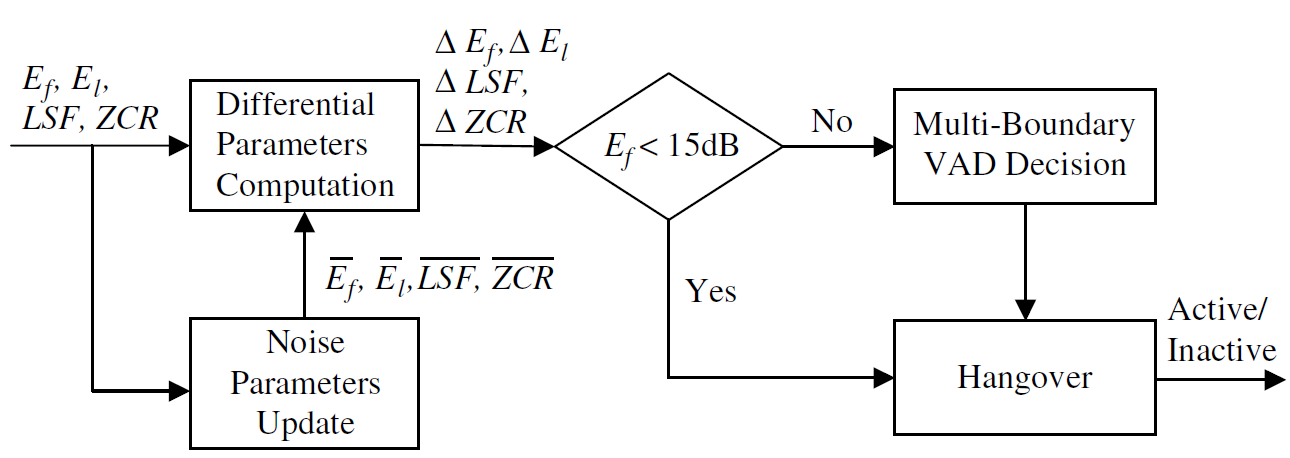
\includegraphics[width=0.9\columnwidth]{Figures/G729AnnexB.png}
		\rule{37em}{0.5pt}
	\caption[Block diagram of the ITU-T G.729 Annex B VAD]{Block diagram of the ITU-T G.729 Annex B VAD \cite{Kondoz}}
	\label{fig:G729AnnexB}
\end{figure}

The \emph{instantaneous parameters} are then differenced with their most recent average noise-only counterparts in order to derive an additional set of so called \emph{difference parameters} which are used for speech/non-speech classification. The set of all possible \emph{difference parameters} describes a four dimensional Euclidean space in which a specific region contains the speech frames while another region describes the noise-only frames. The current vector of parameters is compared against the pre-computed regions in order to classify the current frame. The two regions are initially identified by visual inspection of the points' distribution over a large set of clean and noisy recordings. An energy threshold of $E_f < 15$ dB is applied before the multi-boundary classification in order to minimise short glitches on low-energy frames.

ITU-T G.729 Annex B uses an additional four-step heuristic-based smoothing scheme after the initial multi-boundary classification:
\begin{enumerate}
\item An active voice decision is extended to the current frame if its energy is above a certain threshold
\item An active voice decision is extended to the current frame if the previous two frames were speech and the absolute energy difference between the current and previous frames' is under a certain threshold
\item An inactive voice decision is extended to the current frame if the previous 10 frames were noise-only and the absolute energy difference between current and previous frames' is under a certain threshold
\item The active voice frame is labelled as inactive if the current frame energy is below a noise floor by a certain threshold
\end{enumerate}

The main VAD algorithm also performs updating of the noise parameters ($\overline{LSF}$, $\overline{E_f}$, $\overline{E_l}$ , $\overline{ZCR}$) by a secondary VAD decision which does not need to be as robust as the primary one since it is used only for estimation of the noise parameters.

\subsection{ETSI AMR1 and AMR2}

ETSI proposed two VAD alternatives for use in the Adaptive Multi-Rate speech traffic channels. In both algorithms, the decision is primarily based on the energy of the signal across different frequency bands.

Block diagram of the AMR Option 1 VAD is presented in Figure \ref{fig:AMR1}. The original algorithm includes additional processing steps to those depicted in the Figure in order to determine whether the incoming signal, if not noise-only, contains speech, special information tone (STI) or other (e.g. music), however this details are are omitted in this description.

\begin{figure}[htbp]
	\centering
		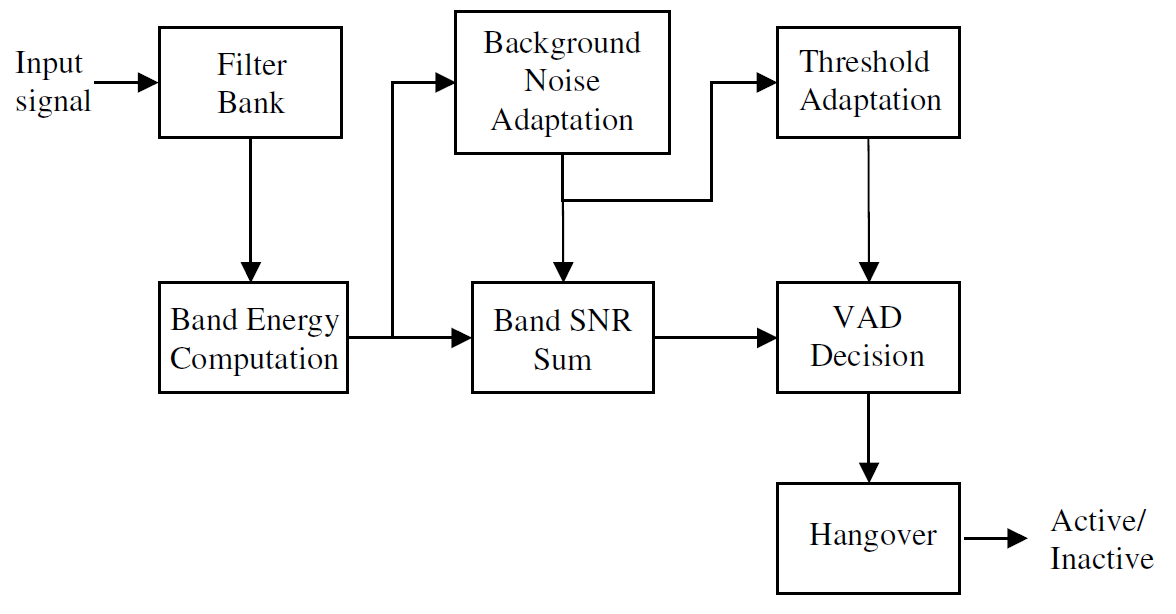
\includegraphics[width=0.9\columnwidth]{Figures/AMR1.png}
		\rule{37em}{0.5pt}
	\caption[Block diagram of the ETSI AMR Option 1 VAD]{Block diagram of the ETSI AMR Option 1 VAD \cite{Kondoz}}
	\label{fig:AMR1}
\end{figure}

The input signal is first passed through a series of nine band-pass filters which split the time-domain signal into different frequency bands based on the Table \ref{tab:AMR1filterbank}. The signal level $level[n]$ is calculated at the output of each filter as a sum of the absolute values of all samples in the current frame. The VAD feature is then computed according to the Equation \ref{eq:AMR1SNR}

\begin{equation}
\text{SNR} = \sum_{n=1}^{9} \max (1.0, \frac{level[n]}{bckr\_est[n]})^{2} 
\label{eq:AMR1SNR}
\end{equation}

where $bckr\_est[n]$ is the estimated level of noise at frequency band $n$. The VAD feature from the above equation is compared to a threshold in order to classify the current frame. The threshold is determined based on the estimated average background noise level which is the sum of $bckr\_est[n]$ for all $n$. As a final processing step, AMR Option 1 VAD includes a hang-over scheme in order to detect the low-energy endings of speech bursts.

\begin{table}[htbp]
\center
\begin{tabular}{c|c|}
\cline{2-2}
 & Frequencies \\ \hline
\multicolumn{1}{ |c| }{Filter 1} & 0 - 250 Hz \\ \hline
\multicolumn{1}{ |c| }{Filter 2} & 250 - 500 Hz \\ \hline
\multicolumn{1}{ |c| }{Filter 3} & 500 - 750 Hz \\ \hline
\multicolumn{1}{ |c| }{Filter 4} & 750 - 1000 Hz \\ \hline
\multicolumn{1}{ |c| }{Filter 5} & 1000 - 1500 Hz \\ \hline
\multicolumn{1}{ |c| }{Filter 6} & 1500 - 2000 Hz \\ \hline
\multicolumn{1}{ |c| }{Filter 7} & 2000 - 2500 Hz \\ \hline
\multicolumn{1}{ |c| }{Filter 8} & 2500 - 3000 Hz \\ \hline
\multicolumn{1}{ |c| }{Filter 9} & 3000 - 4000 Hz \\ \hline
\end{tabular}
\caption[Cut-off frequencies for the ETSI AMR1 band-pass filters]{Cut-off frequencies for the ETSI AMR1 band-pass filters \citep{AMR}}
\label{tab:AMR1filterbank}
\end{table}

Block diagram of ETSI AMR Option 2 VAD is presented in Figure \ref{fig:AMR2}. The concept is similar to Option 1 VAD, however the incoming signal is split into different frequencies not by time-domain band-pass filtering, but by first computing the Discrete Fourier Transform (DFT) of the signal and performing further analysis in the frequency domain. The frequencies are clustered into bands (channels) and the energy of each channel is calculated \citep{Cornu}. In the next processing steps, SNR of each channel is calculated and transformed to a \emph{voice metric} by a specific function which results in the final VAD feature to be classified by using a threshold. An additional part of the system performs updates of the noise statistics based on the spectral deviation estimate.

\begin{figure}[htbp]
	\centering
		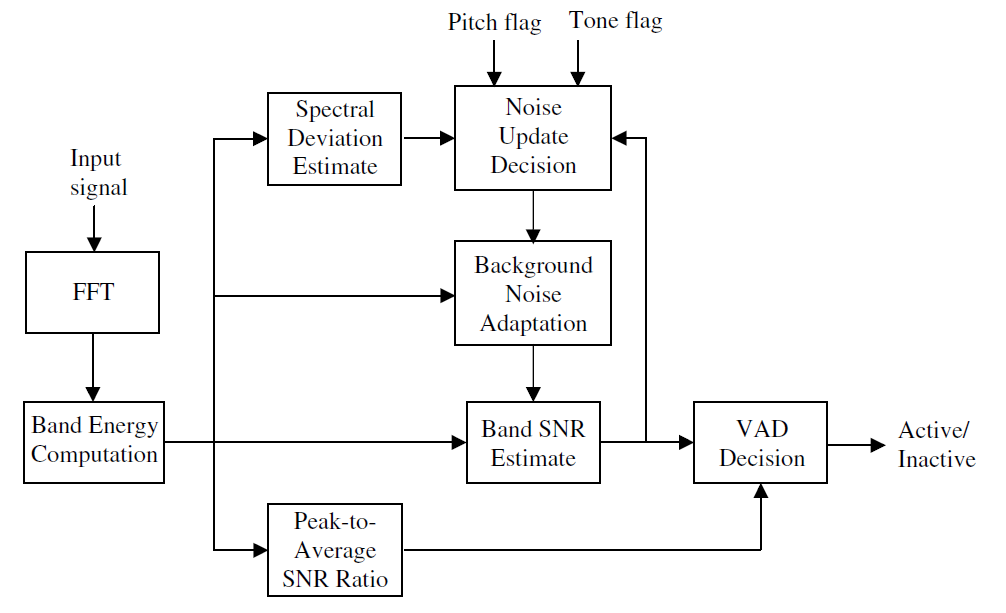
\includegraphics[width=0.9\columnwidth]{Figures/AMR2.png}
		\rule{37em}{0.5pt}
	\caption[Block diagram of the ETSI AMR Option 2 VAD]{Block diagram of the ETSI AMR Option 2 VAD \cite{Kondoz}}
	\label{fig:AMR2}
\end{figure}

\subsection{TIA/EIA IS-733}

TIA/EIA IS-733 is a speech coder in which the signal might be encoded at four different rates (1, 1/2, 1/4, 1/8 of the base rate) depending on the characteristics of the currently transmitted frame. Rate 1 is used for low quality signals where additional reduction might compromise the already low intelligibility. Rate 1/2 is used for good quality stationary and periodic frames. Rate 1/4 is used for unvoiced speech and rate 1/8 for speech inactive frames. A VAD algorithm is used to determine the rate at which the current frame should be encoded and transmitted.

Block diagram of TIA/EIA IS-733 VAD is presented in Figure \ref{fig:IS733}. The algorithm starts with computing the energy of the input signal across two different frequency bands (0.3 - 2.0 kHz and 2.0 - 4.0 kHz) and subsequently the SNR based on the estimated noise energy. The VAD decision is based on two adaptive thresholds, which depend on the level of the estimated background noise, one for each frequency band. If both low and high band SNRs are higher than the threshold, rate 1 is selected. Only one SNR being above its threshold causes the signal to be encoded at rate 1/2. Both SNRs below the threshold indicate noise-only frame, encoded at rate 1/8.

\begin{figure}[htbp]
	\centering
		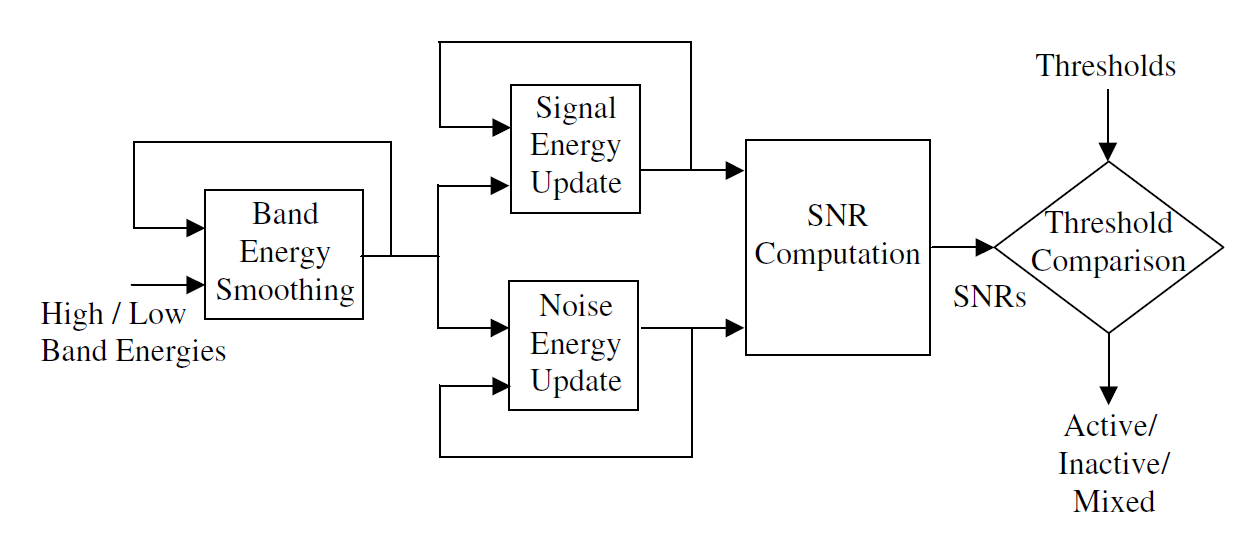
\includegraphics[width=0.9\columnwidth]{Figures/IS733.png}
		\rule{37em}{0.5pt}
	\caption[Block diagram of the TIA/EIA IS-733 VAD]{Block diagram of the TIA/EIA IS-733 VAD \cite{Kondoz}}
	\label{fig:IS733}
\end{figure}

\subsection{Summary}

Some VAD algorithms have been standardised by various telecommunication standards institutes (ITU-T, ETSI, TIA/EIA). Those algorithms are predominantly based on simple features such as the energy of the signal or the zero-crossing rate, sometimes across different frequency ranges. While such measures are often sufficient to meet the requirements of the high SNR transmission found in telecommunications, their performance drops significantly with the increased power of noise. Nevertheless, the standard algorithms serve as a convenient benchmark for the more recently proposed VADs, described in section \ref{sec:RobustVADs} which are aimed to be more noise-robust and useful in other speech processing tasks.

%----------------------------------------------------------------------------------------
%	SECTION 2 - Noise-robust VAD algorithms
%----------------------------------------------------------------------------------------

\section{Noise-robust VAD algorithms}
\label{sec:RobustVADs}

Apart from standard VAD algorithms described in section \ref{sec:StandardVADs}, many independent researchers have made numerous attempts to develop novel noise-robust Voice Activity Detection methods. Most of these research results either in invention of the new features or identification of ways in which the existing ones might be improved. Ideally, the most robust feature should have no common values for the noise and speech frames. Figure \ref{fig:featureDist} shows the distribution of values for some of the features used by algorithms described in this section for the clean speech from the TIMIT \cite{TIMIT} database and a variety of noise types from the NOISEX-92 \cite{NOISEX} database. It is clear, that in both cases the values for the clean speech are mostly distinct from the ones for noise frames, however there is still much overlap between them which indicates a room for improvement.

\begin{figure}[htbp]
	\centering
		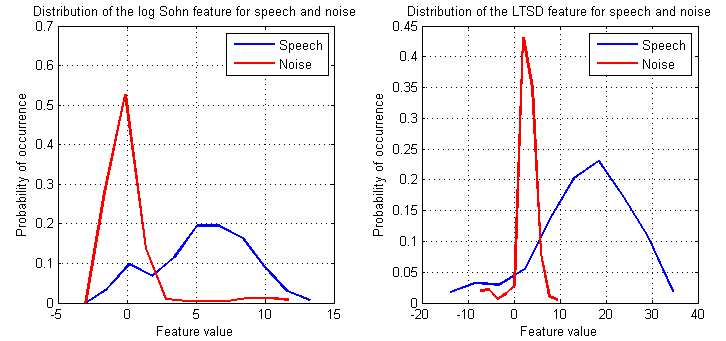
\includegraphics[width=0.9\columnwidth]{Figures/featureDist.png}
		\rule{37em}{0.5pt}
	\caption[Distribution of Sohn's and LTSD features for speech and noise]{Distribution of Sohn's \cite{SohnInitial} and LTSD \cite{LTSD} features for speech and noise}
	\label{fig:featureDist}
\end{figure}

\subsection{Entropy-based VADs}

In contrast to the standardised energy-based methods, some researchers investigated the idea of using entropy for Voice Activity Detection. Entropy, as originally defined by Shannon \cite{Shannon}, is a measure of uncertainty in a random variable, given by the equation:

\begin{equation}
E = - \sum_{i=1}^{N} p_i \log_2 p_i
\label{eq:entropy}
\end{equation}

where $p_i$ is the probability of the random variable having a value of $i$ among $N$ distinct values which it might take. In case of VAD, $p_i$ often relates to either a single bin in a histogram of the amplitudes of a signal or a single frequency in the magnitude or power spectrum.

The purely time domain approach to VAD using entropy has been explored by Weaver \emph{et al.} in \cite{Weaver}. Block diagram of the key parts of the algorithm is presented in Figure \ref{fig:Weaver}. Authors propose to first calculate the histogram of the amplitudes of the signal and then assign an entropy measure to each frame, as defined in Equation \ref{eq:entropy}, where $p_i$ is the normalised (such that $\sum_{i=1}^{N} p_i = 1$) mass of the $i$-th bin of the histogram.

\begin{figure}[htbp]
	\centering
		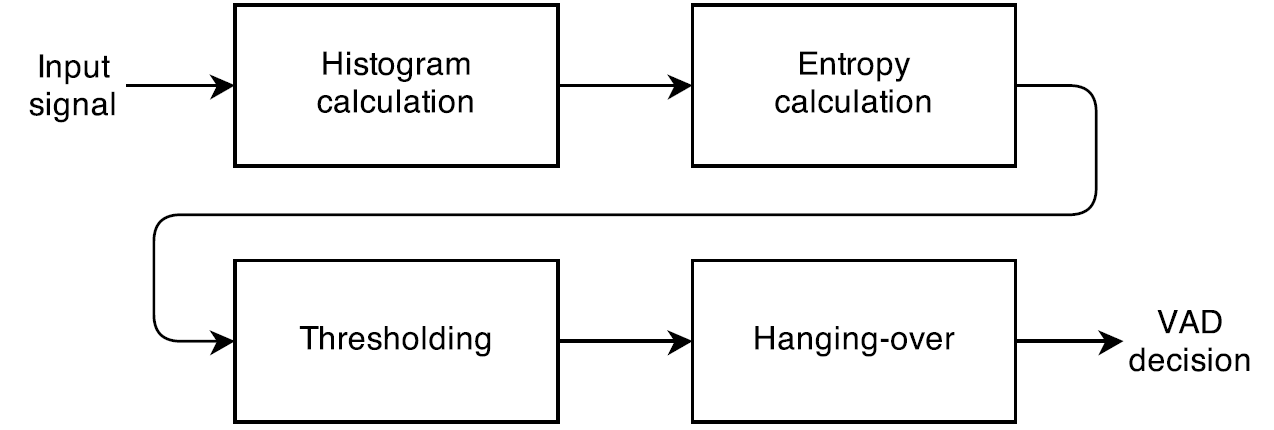
\includegraphics[width=0.9\columnwidth]{Figures/Weaver.png}
		\rule{37em}{0.5pt}
	\caption[Block diagram of the time-domain entropy-based VAD]{Block diagram of the time-domain entropy-based VAD \cite{Weaver}}
	\label{fig:Weaver}
\end{figure}

While this approach is more noise-robust than the simple energy-based methods, especially for the stationary narrowband noise types, its performance is significantly affected by the various coloured noises. In order to mitigate this weakness, authors propose to use a weighting filter in order to enhance the typical speech frequencies, however it needs to be kept in mind that if we are faced with a noise with spectral characteristics very similar to speech (especially in case of the \emph{babble noise}), the filter would become essentially useless as it would emphasise the noise as well.

A frequency domain approach to using entropy for VAD has been considered by Renevey \emph{et al.} in \cite{Renevey}. Instead of first computing the histogram of the amplitudes of the input signal, the frequency-domain algorithm starts with calculating the power spectrum of each frame. Entropy of the spectrum is then calculated by means of the following equation:

\begin{equation}
E( \left |  Y \left ( \omega, t \right ) \right |^{2} ) = - \sum_{i=1}^{L} P( \left |  Y \left ( \omega_i, t \right ) \right |^{2} ) \log \left( P( \left |  Y \left ( \omega_i, t \right ) \right |^{2} ) \right)
\end{equation}

where $P( \left |  Y \left ( \omega_i, t \right ) \right |^{2} )$ denotes the fraction of the sum of all harmonics which is attributable to the current frequency $i$.

\begin{figure}[htbp]
	\centering
		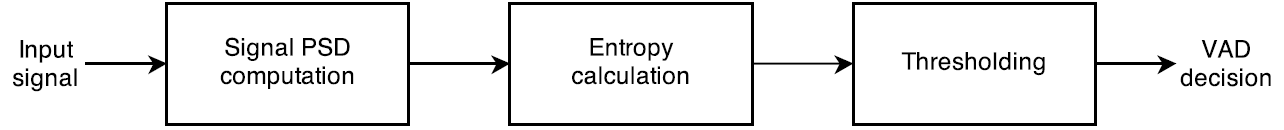
\includegraphics[width=0.9\columnwidth]{Figures/Renevey.png}
		\rule{37em}{0.5pt}
	\caption[Block diagram of the frequency-domain entropy-based VAD]{Block diagram of the frequency-domain entropy-based VAD \cite{Renevey}}
	\label{fig:Renevey}
\end{figure}

All entropy-based approaches to VAD are most effective for the white noise and alike, since the distribution of entropy for speech is much different from the one for noise. The completely unpredictable nature of white noise yields high entropy values, while the more organised and predictable clean speech signals present a naturally lower entropy. Both the time and frequency domain algorithms' performance drops significantly for a variety of coloured noise types. In order to improve the performance for in such environments, authors of \cite{Renevey} propose using a \emph{whitening} filter which divides the spectrum of the current frame by an average of all frames.

\subsection{Likelihood Ratio Test VADs}
\label{ssec:LRT}

'A Statistical Model-Based Voice Activity Detector' proposed by Sohn \emph{et al.} \cite{Sohn} is one of the most widely cited VAD algorithms due to its ease of implementation, robustness and extensibility. The idea of using a Likelihood Ratio Test (LRT) has been considered by many other researchers who tried to improve on the original approach \cite{ImprovedLikelihood, Cho}. The initial algorithm has been developed in \cite{SohnInitial} and extended to improve noise-robustness in \citep{Sohn}. Block diagram of Sohn's VAD is presented in Figure \ref{fig:Sohn}.

\begin{figure}[htbp]
	\centering
		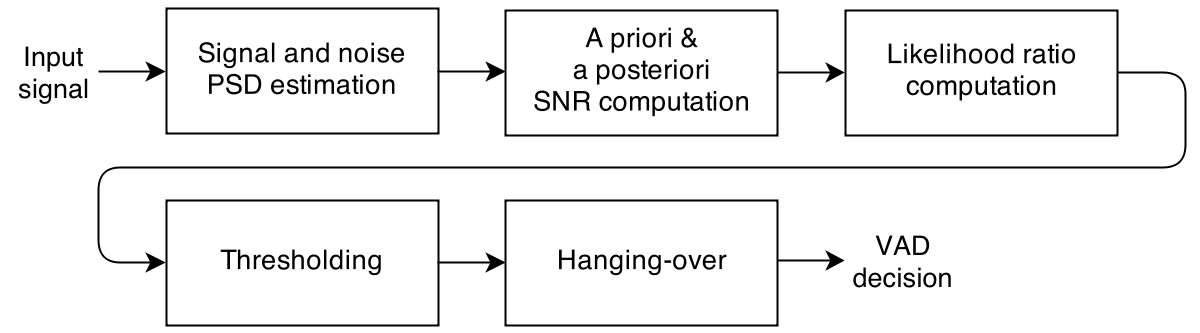
\includegraphics[width=0.9\columnwidth]{Figures/Sohn.png}
		\rule{37em}{0.5pt}
	\caption[Block diagram of the Statistical Model-Based VAD]{Block diagram of the Statistical Model-Based VAD \cite{Sohn}}
	\label{fig:Sohn}
\end{figure}

The algorithm is based on a LRT to discriminate between two hypotheses:
\begin{itemize}
\item[] $H_0$ - speech absent
\item[] $H_1$ - speech present
\end{itemize}

The measure which is used for the preliminary VAD decision (i.e. before the hang-over scheme) is a combination of the likelihood ratios from each frequency bin $k$:

\begin{equation}
\log \Lambda = \frac{1}{L} \sum_{k=0}^{L-1} \log \frac{1}{1+\xi_k} e^{\frac{\gamma_k\xi_k}{1+\xi_k}}
\end{equation}

where $L$ is the number of samples in each frame, $\xi_k$ is the \emph{a priori} SNR and $\gamma_k$ is the \emph{a posteriori} SNR. In order for the algorithm to work, one needs to obtain the values for $\xi_k = \frac{\left | S_k \right |^{2}}{\left | N_k \right |^{2}}$ and $\gamma_k = \frac{\left | X_k \right |^{2}}{\left | N_k \right |^{2}}$ where $\left | X_k \right |^{2}, \left | S_k \right |^{2}, \left | N_k \right |^{2}$ are the PSDs of the noisy speech, clean speech and noise respectively. $\left | N_k \right |^{2}$ can be obtained by means of any noise estimation procedure (e.g. \cite{MSnoise} or \cite{MMSEnoise}), whose accuracy influences the noise robustness of the algorithm. The VAD feature is thresholded by an empirically determined constant for the preliminary decision. Finally, authors proposed a Hidden Markov model (HMM) hang-over scheme in order to improve accuracy of the algorithm for the low-energy beginnings and endings of the speech utterances.

While the original idea to the derivation of the unknown \emph{a priori} SNR $\xi_k$ involved the Maximum Likelihood estimator $\xi_k^{ML} = \gamma_k - 1$, in \cite{Sohn} a limitation of the procedure has been identified which makes it biased towards $H_1$. In an effort to improve the algorithm, authors proposed a decision-directed (DD) estimation procedure which reduces the fluctuation of the likelihood ratios by using a MMSE short-time spectral amplitude estimator \cite{Ephraim} and a first-order low pass filter.

In an effort to further improve the LRT-based algorithm, Cho \emph{et al.} \cite{Cho} investigated the DD approach with particular interest in the detection errors occurring at the endings of speech utterances. It was determined that the frequent misdetections are due to the delay in the DD \emph{a priori} SNR estimator, which prevents the estimated value to drop quick enough for the likelihood ratio to stay above the threshold during the short, low-energy speech offset regions. In order to alleviate this problem, authors proposed a smoothed likelihood ratio (SRT), which delays the sudden drops in the LR at the speech offset regions due to the constant $\alpha \approx 0.9$. The SRT is defined in Equation \ref{eq:SRT} where $n$ relates to the frame number while $k$ is the frequency bin. The final VAD decision is calculated by taking a geometric mean of the SRTs from all frequency bins.

\begin{equation}
\Phi (n,k) = \exp \left\{ \alpha \log \left( \Phi (n-1,k) \right) + (1-\alpha) \log \left( \Lambda (n,k) \right) \right\}
\label{eq:SRT}
\end{equation}

Both \cite{Sohn} and \cite{Cho} VADs consider only a single frame when making a speech/non-speech decision and hence they are likely to misclassify the low-energy frames for which the short-time SNR is much lower than the average SNR of the entire signal. To aid the proper detection of such frames, in \cite{RamirezMulti} Ramirez \emph{et al.} proposed a multiple observation vector which considers $M$ frames before and ahead of the current frame in formulating the likelihood ratio. The main rationale behind this idea is that the weaker speech frames are often surrounded by the stronger parts, and their inclusion in the LRT might boost its value above the threshold. While this approach results in somewhat improved performance, it also introduces the delay of $M$ frames to the algorithm, which might prevent it from being used in some real-time applications.

\subsection{Long-Term Spectral Divergence VAD}

Another popular and widely cited algorithm is the Ramirez \emph{et al.} \cite{LTSD} VAD based on the long-term speech information. The main assumption of the algorithm is that the most discriminative speech/non-speech information lies on the shape of the magnitude spectrum of the analysed signal. However, instead of considering each frame independently, the algorithm also includes the information contained in the neighbouring frames. The reason behind that is to boost the detection of the low-energy unvoiced phonemes which are typically surrounded by the high-energy voiced ones. Therefore, it can be said that the LTSD algorithm uses an implicit hang-over scheme incorporated directly in the voicing feature.

The algorithm starts by computing the so-called long-term spectral envelope (LTSE) which uses information contained in the current frame as well as $N$ preceding and succeeding frames i.e. $2N+1$ frames in total for every calculation. Based on the LTSE, the long-term spectral divergence (LTSD) is calculated which serves as the VAD decision rule. In Ramirez's study, it has been established that the best performance is achieved for $N=6$ however this value is likely to be dependent on the particular application as well as the level of noise.

\begin{figure}[htbp]
	\centering
		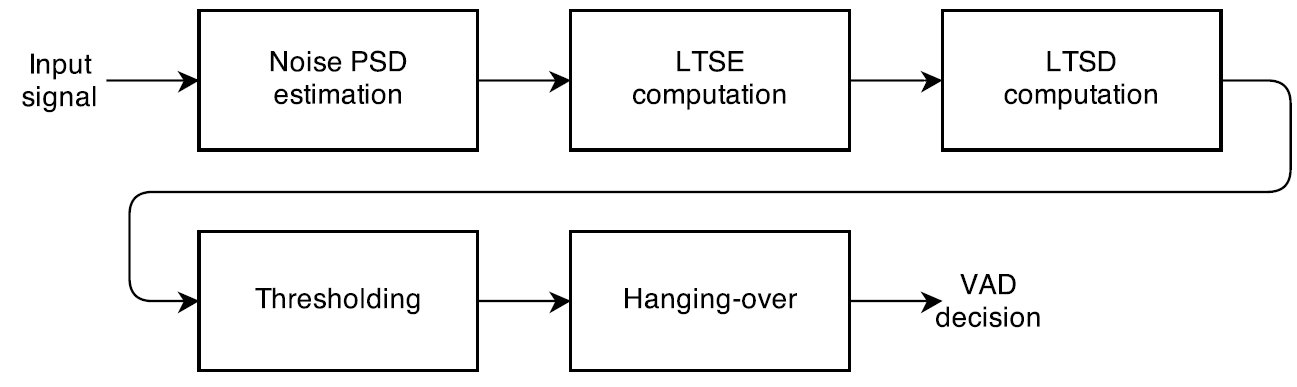
\includegraphics[width=0.9\columnwidth]{Figures/LTSD.png}
		\rule{37em}{0.5pt}
	\caption[Block diagram of the Long-Term Spectral Divergence VAD]{Block diagram of the Long-Term Spectral Divergence VAD \cite{LTSD}}
	\label{fig:LTSD}
\end{figure}

Block diagram of the LTSD-based VAD is presented in Figure \ref{fig:LTSD}. The algorithm starts with an assumption that the first $N$ frames of each utterance do not contain any speech and that the average magnitude spectrum of the noise can be estimated from them. After that, the LTSE for each frame is computed according to Equation \ref{eq:LTSE} where $X(k,l)$ is the amplitude spectrum at frequency $k$ for frame $l$.

\begin{equation}
\text{LTSE}(k,l) = \max \left \{ X(k,l-N),\ldots,X(k,l),\ldots,X(k,l+N) \right \}
\label{eq:LTSE}
\end{equation}

The LTSD is obtained from Equation \ref{eq:LTSD} where $M$ is the number of frequency bins in the DFT and $N(k)$ is the average noise amplitude spectrum at frequency $k$ as estimated before. Essentially what the equation describes is the average deviation of the LTSE from the noise statistics at each frequency bin. In other words, this measure might be interpreted as a variation of the estimated \emph{a posteriori} signal-to-noise ratio, which is an idea exploited in many VAD algorithms.

\begin{equation}
\text{LTSD}(l) = 10 \log_{10} \left ( \frac{1}{M} \sum_{k=0}^{M-1} \frac{\text{LTSE}^{2}(k,l)}{N^{2}(k)} \right )
\label{eq:LTSD}
\end{equation}

Eventually, the LTSD feature is thresholded to form a preliminary VAD decision which might be further revised by a separate hang-over scheme.

\subsection{Pitch and fundamental frequency based VADs}

A rather unique feature of voiced speech is its spectral harmonicity. The magnitude spectrum of voiced phonemes contains clearly visible peaks at equal intervals corresponding to the fundamental frequency $F_0$ or pitch, terms which in speech processing context are often used interchangeably. A spectrogram of a sample utterance corrupted by 0 dB car noise is presented in Figure \ref{fig:harmospgramcar}. Although the energy of the noise is high (making the speech detection a challenge for the energy-based algorithms), its PSD occupies mostly the low frequencies (yellow box) causing the harmonic peaks (red boxes) to remain undistorted. Even in the presence of 0 dB white noise (Figure \ref{fig:harmospgramwhite}), which is much richer in frequency components than car noise, the harmonic peaks are preserved, although to a much smaller extent. While it is clearly possible to use the harmonicity features for the detection of the voiced parts of speech utterances, the unvoiced phonemes' spectrum does not contain harmonic peaks. Therefore, detection of the unvoiced phonemes remains difficult and often requires an additional technique or a specialised hang-over scheme.

\begin{figure}[htbp]
	\centering
		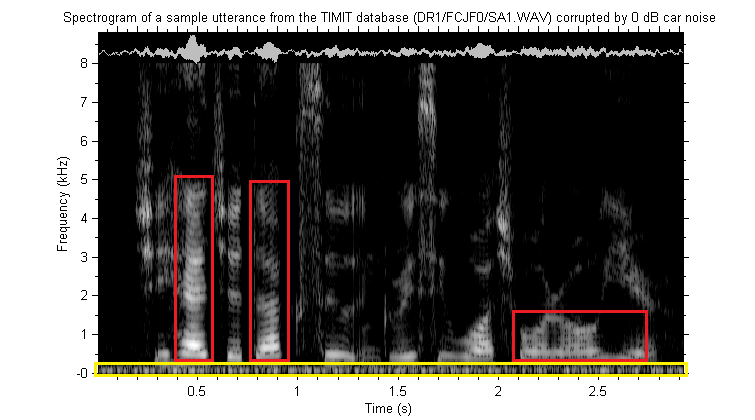
\includegraphics[width=0.9\columnwidth]{Figures/harmospgramcar.png}
		\rule{37em}{0.5pt}
	\caption[Spectrogram of a sample utterance corrupted by 0 dB car noise]{Spectrogram of a sample utterance corrupted by 0 dB car noise}
	\label{fig:harmospgramcar}
\end{figure}

\begin{figure}[htbp]
	\centering
		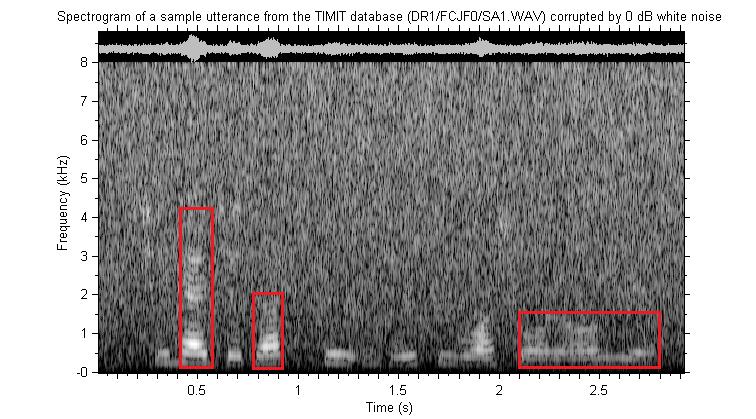
\includegraphics[width=0.9\columnwidth]{Figures/harmospgramwhite.png}
		\rule{37em}{0.5pt}
	\caption[Spectrogram of a sample utterance corrupted by 0 dB white noise]{Spectrogram of a sample utterance corrupted by 0 dB white noise}
	\label{fig:harmospgramwhite}
\end{figure}

In \cite{PARADE} Ishizuka \emph{et al.} proposed a VAD (dubbed PARADE) based on the ratio of the powers of periodic to aperiodic components of the signal. Block diagram of the algorithm is presented in \ref{fig:PARADE}. The VAD decision is based on the likelihood ratio defined in Equation \ref{eq:PARADE} where $\phi (i)$ equals $\frac{\hat{\lambda}_p (i)}{\hat{\lambda}_a (i)}$ - the ratio of the average power per frequency bin of the periodic to aperiodic components of the signal in frame $i$.

\begin{equation}
\Lambda(i) = \frac{1}{\phi (i)} \exp \left\{ \frac{1}{2} \left( \phi (i)^{2} - \frac{1}{\phi (i)^{2}} \right) \right\}
\label{eq:PARADE}
\end{equation}

The authors propose to approximate the average powers from Equations \ref{eq:aperiodicpower} and \ref{eq:periodicpower} where $\vartheta$ is the number of harmonics in the current frame and $\eta$ is a specific constant for power estimation.

\begin{equation}
\hat{\lambda}_a = \frac{\lambda - \eta \sum_{m=1}^{\vartheta} \left| X(m f_0) \right|^{2}}{1-\eta \vartheta}
\label{eq:aperiodicpower}
\end{equation}

\begin{equation}
\hat{\lambda}_p = \lambda - \hat{\lambda}_a
\label{eq:periodicpower}
\end{equation}

\begin{figure}[htbp]
	\centering
		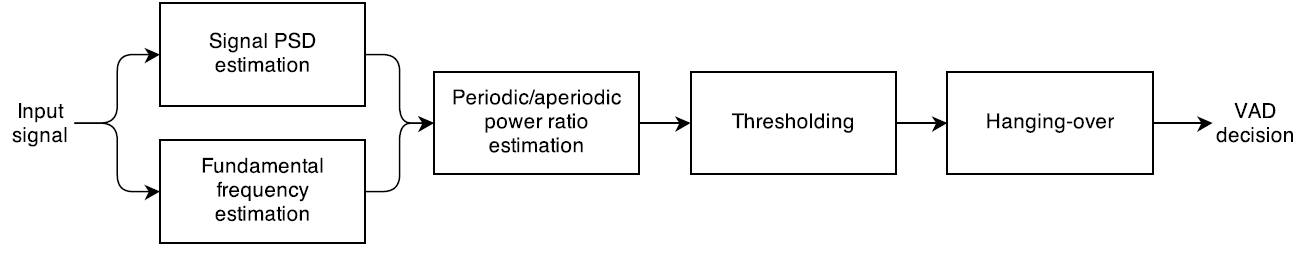
\includegraphics[width=0.9\columnwidth]{Figures/PARADE.png}
		\rule{37em}{0.5pt}
	\caption[Block diagram of the periodic/aperiodoc component ratio VAD]{Block diagram of the periodic/aperiodoc component ratio VAD \cite{PARADE}}
	\label{fig:PARADE}
\end{figure}

While this concept is likely to be robust to various non-stationary noise types, by definition it cannot cope with the unvoiced parts of speech, detection of which has to be performed by a hang-over scheme. In the original paper, authors did not specify how to estimate the number of harmonics $\vartheta$ for each frame, which is crucial to the proper working of the algorithm. A potential improvement might also come from an improved pitch detection method.

Another approach to using harmonic frequency components\footnote{This algorithm also builds on the idea of LRT described in section \ref{ssec:LRT}. The main improvement comes however from utilising the spectral harmonicity therefore it has been included in this section} for VAD has been investigated by Tan \emph{et al.} in \cite{Tan}. The authors claim, that under low SNR the approach from \cite{RamirezMulti} is likely to fail since the LRs from the high-energy frames will not be strong enough to aid the proper classification of the low-energy frames. Therefore, they propose a new way of calculating the LRs for the voiced frames, defined in Equation \ref{eq:harmfreq} where $\vartheta$ is the number of harmonics within the resolution of the DFT and $f_0$ denotes the fundamental frequency. The algorithm calculates the LR only using the frequency bins which are multiples of the fundamental frequency.

\begin{equation}
\log \Lambda_v = \frac{1}{\vartheta} \sum_{m=1}^{\vartheta} \log \Lambda(m f_0)
\label{eq:harmfreq}
\end{equation}

Voiced frames are pre-identified by the pitch determination algorithm, and all others are considered as unvoiced. The LR for the unvoiced frames is calculated in a standard way from \cite{SohnInitial} i.e. by considering all frequency bins.

\subsection{Summary}

Voice Activity Detection has been studied by numerous researchers over the recent years. Some of the most simple features proposed in the literature, apart from energy, are based on the entropy of the signal, either in time or frequency domain.

The popular LRT based approach, initially proposed by Sohn \emph{et al.}, has served as a basis for many researchers who tried to improve the original algorithm. While Sohn \emph{et al.} employed the LRT to the SNR, the idea has also been applied to other features, such as the periodic to aperiodic component ratio. Nevertheless, many VAD algorithms still utilise the estimated SNR as a voicing feature. Ramirez \emph{et al.} proposed one such VAD, where the SNR is calculated for a given frame including information from the neighbouring frames, rather than considering each frame independently.

The most noise-robust VAD algorithms are likely to be the ones which are based on the harmonicity of the speech signal. Since voiced speech typically does not present high energy in all frequency bins, it is beneficial to first identify the fundamental frequency of a signal and consider the power around the multiples of it. While this approach inherently cannot detect the aperiodic unvoiced phonemes, a clever hang-over scheme can help in their proper classification, by extending the initial VAD decisions to include such misdetected speech segments.

%----------------------------------------------------------------------------------------
%	SECTION 3 - Conclusion
%----------------------------------------------------------------------------------------

\section{Conclusion}

This chapter presented a literature survey of the most commonly encountered approaches to Voice Activity Detection. In section \ref{sec:StandardVADs} some standard algorithms have been described while section \ref{sec:RobustVADs} reviewed the recent research efforts in the VAD area.

In terms of noise-robustness, the standard algorithms are unlikely to achieve satisfactory performance under low SNR conditions since they are primarily based on features such as the energy or the zero-crossing rate which are easily degradable by high background noise levels. In such conditions, performance of the recently proposed VAD algorithms is expected to be much better.